\begin{frame}
  \frametitle{Convolutional Neural Networks}
  \begin{itemize}
    \item Simple ANNs work well for moderate amounts of features
      \begin{itemize}
        \item Problems arise when amount of features grows
        \item Number of parameters (weights and biases) ``explodes''
        \item Requires huge amounts of space and nearly impossible to
          train
      \end{itemize}
    \item Sometimes, the input has a specific structure
      \begin{itemize}
        \item E.g. images are arranged in grids of pixels (fault
          heatmaps are similar)
        \item Every pixel has a \textit{local} relevance
        \item No need to connect every neuron to every input
      \end{itemize}
    \item Use that structure to create simpler models that are easier
      to train
  \end{itemize}
\end{frame}

\begin{frame}
  \frametitle{Convolution Layers}
  \begin{itemize}
    \item Arrange the neurons in a grid, just like the input
    \item Every neuron ``watches'' a specific area, the \textit{local
      receptive field}
      \begin{itemize}
        \item Weights are shared \(\rightarrow\) less parameters
      \end{itemize}
    \item Works just like a sliding window (similar to a
      \textit{convolution})
    \item Multiple convolutions are performed \(\rightarrow\) stack of
      hidden grids
  \end{itemize}
  \begin{figure}
    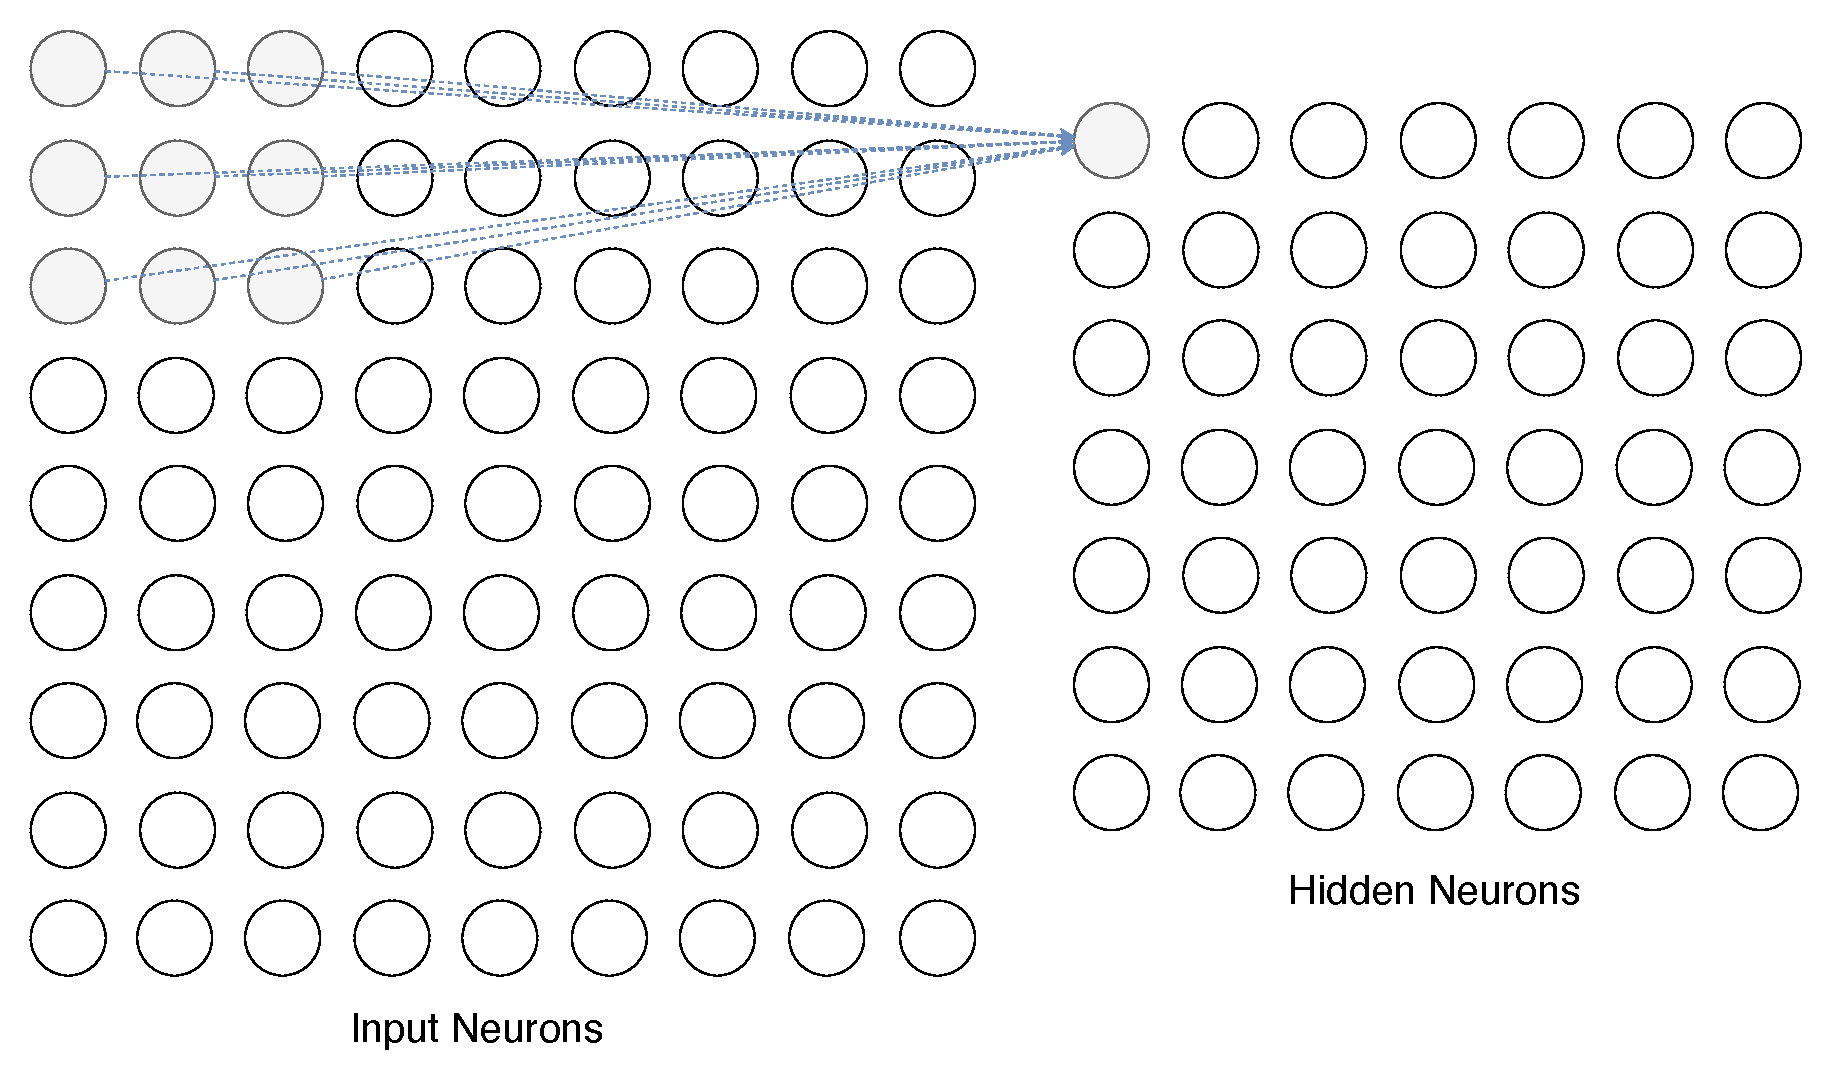
\includegraphics[width=.7\textwidth]{../figures/receptive_field}
  \end{figure}
\end{frame}

\begin{frame}
  \frametitle{Pooling Layers}
  \begin{itemize}
    \item Reduce the input's complexity by downsampling
      \begin{itemize}
        \item Every neuron just remembers the maximum of its local
          receptive field
      \end{itemize}
    \item Forget about the exact location of a feature
      \begin{itemize}
        \item Leads to \textit{spatial invariance}
      \end{itemize}
  \end{itemize}
  \begin{figure}
    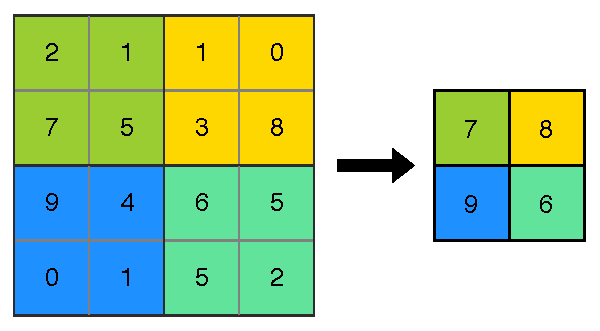
\includegraphics[width=.55\textwidth]{../figures/pooling}
  \end{figure}
\end{frame}

\begin{frame}
  \frametitle{The Convolutional Architecture}
  \begin{itemize}
    \item Stack multiple convolution and pooling layers
      \begin{itemize}
        \item These are used to extract relevant features
      \end{itemize}
    \item Use a fully connected layer in the end to perform
      classification
    \item The network is also trained via \textit{gradient descent}
      \begin{itemize}
        \item Weights and biases are updated in each step to minimize
          classification error
      \end{itemize}
  \end{itemize}
  \begin{figure}
    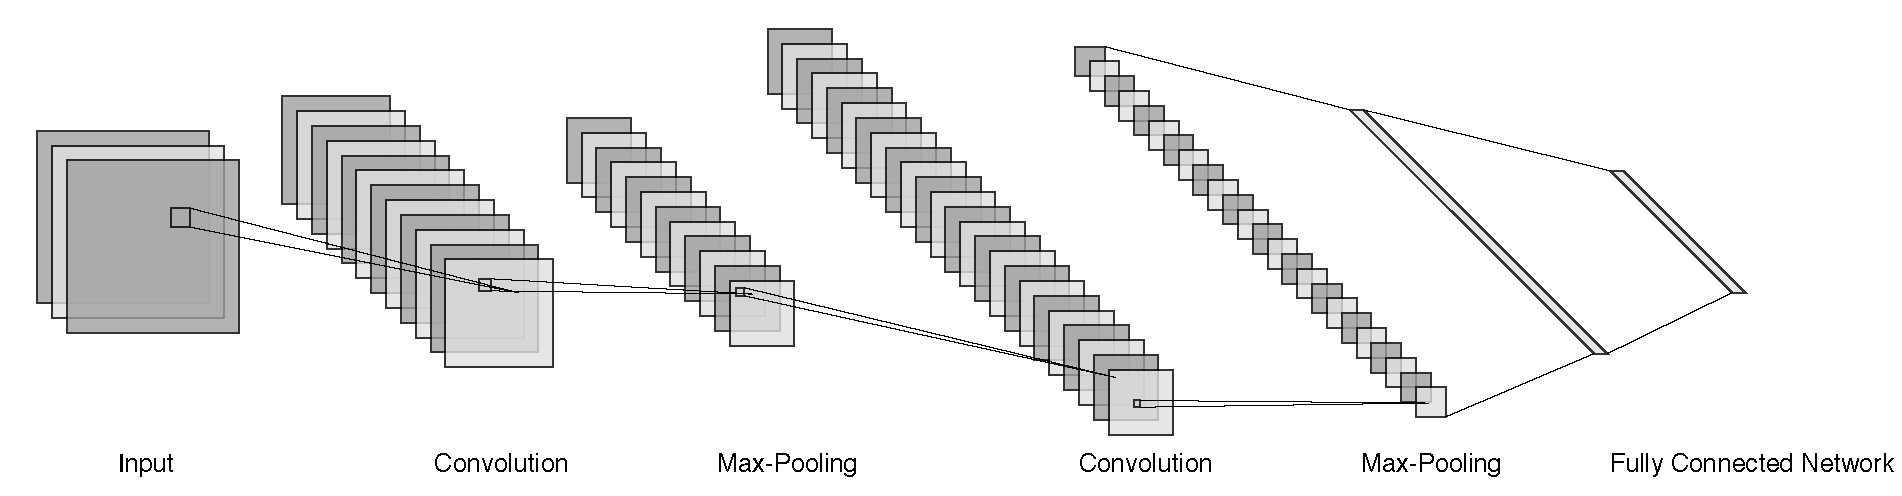
\includegraphics[width=\textwidth]{../figures/convnet}
  \end{figure}
\end{frame}
